% -------------------------------------------------------------
%		Preamble
%--------------------------------------------------------------
% !TeX spellcheck = uk_UK
%Document Settings
\documentclass[a4paper,11pt]{scrartcl}
\usepackage[T1]{fontenc}
\usepackage{setspace}
\onehalfspacing
\DeclareOldFontCommand{\bf}{\normalfont\bfseries}{\mathbf} % Includes an old command that is part of some package in here (just to make sure erverything runs)

% Page numbers
\newcommand{\sectionnumbering}[1]{%
  \setcounter{section}{0}%
   \renewcommand{\thesection}{\csname #1\endcsname{section}}}

% Language settings
\usepackage[utf8]{inputenc}
\usepackage[english]{babel}

% Maths settings
\usepackage{amsmath}
\newcommand\numberthis{\addtocounter{equation}{1}\tag{\theequation}}
\usepackage{amssymb}
\usepackage{siunitx}

% Graphics packages
\usepackage{graphicx}
\graphicspath{{Graphics/}}
\usepackage{adjustbox}

% Table packages
\usepackage{pdflscape} %To create landscape environments
\usepackage{booktabs,caption}
\usepackage{threeparttable} %For nice tables
\usepackage{csvsimple} %To import excel tables 
\usepackage{import}

% Bilbiography settings
\usepackage{natbib}
\bibliographystyle{apalike}


% -------------------------------------------------------------
%		Title Page
%--------------------------------------------------------------
\begin{document}

	\begin{titlepage}
		\newcommand{\HRule}{\rule{\linewidth}{0.5mm}}
		
%% Logo
	\vfill\vfill
	
\includegraphics[height=1.5cm]{UoN_Logo}\\[1cm] 


	\center			
%% Heading
	\textsc{\LARGE University of Nottingham}\\[1.5cm] 
	\textsc{\Large Applied Microeconometrics}\\[0.5cm] 	
	\textsc{\large Group Project A}\\[0.5cm] 
	
%% Title
	\HRule\\[0.4cm]
	{\huge\bfseries Insert Title}\\[0.4cm] 
	\HRule\\[0.4cm]
	
%% Date
	{\large\ Spring Term 2020} 	
	\vfill\vfill\vfill 		
	
%% Author(s) and Supervisor
\begin{flushleft}
			\large
			\textit{Supervisor}\\
			Professor Sourafel \textsc{Girma} 
			\vfill\vfill 
			\textit{Authors}\\
			Nelly  \textsc{Lehn} (20214338)\\
			Yonesse \textsc{Paris} (20115536)\\
			Thea  \textsc{Zoellner} (20216019)\\
			Georg  \textsc{Schneider} (20214032)\\
			Emilie \textsc{Bechtold} (20214031)
		\end{flushleft}
	\vfill 
	
\end{titlepage}


% -------------------------------------------------------------
%		Contents
%--------------------------------------------------------------
\pagenumbering{roman}
\sectionnumbering{Roman}
\tableofcontents

\newpage

\listoftables
\newpage

%-------------------------------------------------------------
% Main Body
%-------------------------------------------------------------
\pagenumbering{arabic}
\sectionnumbering{arabic}

\section{Introduction}



\section{Theoretical Background/Literature Review}

\subsection{FDI}

\subsection{PSM}
Since (I guess) we will be focussing on ATE rather than ATT, we need to satisfy the following two assumptions: 

\begin{enumerate}
\item Assumption: \textbf{Unconfoundedness (CIA)} \\
"\textit{[G]iven a set of observable covariates X which are not affected by treatment, potential outcomes are independent of treatment assignment}"   \citep[p.~35]{CaliendoHujerThomsen2008}	 

\item Assumption: \textbf{Overlap} \\
"\textit{persons with the same X values have a positive probability of being both participants and nonparticipants}" \citet [p.~35]{Caliendo08}

\end{enumerate}
--> if Assumption 1 holds, all biases due to observable components can be removed by conditioning on the propensity score (Imbens, 2004).

\subsubsection*{Binary Treatment}
Difference between logit and probit lies in the link function. Logit assumes a log-distribution of residuals, probit assumes a normal distribution. Heteroskedastic probit models can account for non-constant error variances --> Check for heteroskedasticity?

\subsubsection*{Multiple Treatments}
The multinomial probit model is the preferable option compared to logit. Alternatively, just run several binary ones (more complicated but also more robust to errors).

\subsubsection*{Variable selection}
\begin{itemize}
\item outcome variable must be independent of treatment conditional on the pscore (CIA)
\item Only variables that influence simultaneously the participation decision and the outcome variable should be included (based on theory and empirical findings)
\item variables should either be fixed over time or measured before participation (include only variables unaffeted by participation)
\item choice of variables should be based on economic theory and previous empirical findings
\end{itemize}

\subsubsection*{Tests for variable selection}
Strategies for the selection of variables to be used in estimating the propensity score: ...


\section{Data and Descriptive Analysis}
Our analysis is based on observational firm-level data. The dataset comprises 11,323 firms, of which 4,460 received FDI in 2016. The FDI can be divided into three subcategories. Table \ref{tab:freq} shows the frequencies of each type of FDI in our sample. Among the recipients of FDI, most firms (1,965) received domestic market seeking FDI. 1,555 firms received technology intensive FDI and the remaining 640 firms received exports oriented FDI. The TFP outcome was measured in 2017. We standardize\footnote{Using Z-score standardization} the outcome variable to make its interpretation more intuitive.

%--------------------TABLE 1
\begin{table}[h]
	\centering
	\caption{Frequency of FDI Types} 
	\begin{threeparttable}
\begin{tabular}{lcc} 
	\toprule \toprule 
	FDI type&Abs. Freq.&Rel. Freq. \\[1ex]
	\midrule
	No FDI							& 6,863		& 61\% \\
	Exports oriented FDI			& 940		& 8\%	\\
	Technology intensive FDI 		& 1,555 	& 14\% 	\\
	Domestic market seeking FDI 	& 1,965 	& 17\% 	\\\\[-1.8ex]
	Total 							& 11,323 	& 100\% \\
	\bottomrule \bottomrule
\end{tabular}
\end{threeparttable}
\label{tab:freq}
\end{table}
%---------------------------

A set of categorical and continuous control variables was measured in 2015 (one year prior to the firms receiving FDI). Table \ref{tab:cat} provides an overview of the categorical variables and the frequencies of each category in our sample. The categorical variables are included as factor variables in the subsequent analysis. The port variable indicates whether a firm has access to a port within 500km. The legal ownership of a firm is captured in the ownership variable, where state owned firms represent the base group. The technology intensity of the industry the respective firm is operating in, is measured in four categories from low- to high-tech, low-tech being the base group. The R\&D dummy indicates whether a firm has invested in Research and Design in 2015. \\

%-------------------------TABLE 2
\begin{table}[h]
	\centering
	\caption{Summary Statistics of Categorical Covariates} 
	\begin{threeparttable}

\begin{tabular}{lcc} \toprule \toprule 
			& Abs. Freq.	& Rel. Freq. \\
	\midrule 							\\[-1.8ex]
\textbf{Port}\textsuperscript{a} & & 						\\
No				& 7,366		& 65.05		\\
Yes				& 3,957     & 34.95		\\[1.2ex]
\textbf{Ownership}	& &					\\
Listed company	& 909 		& 8.03 		\\
Subsidiary		& 2,630 	& 23.23 	\\
Independent 	&  4,593 	& 40.56 	\\
State owned		& 3,191     & 28.18		\\[1.2ex]
\textbf{Technology Intensity}	& &		\\
Low-tech		& 4,194		& 37.04 	\\
Medium low-tech	& 1,685		& 14.88 	\\
Medium high-tech & 3,539	& 31.25 	\\
High-tech  		& 1,905		& 16.82 	\\[1.2ex]
\textbf{R\&D}\textsuperscript{b}	& &						\\
No				&  9,951	& 87.88		\\
Yes				& 1,372		& 12.12 	\\[1.2ex]
	\hline \hline
\end{tabular}

\begin{tablenotes}[flushleft]
\footnotesize
\item \textsuperscript{a} Indicates whether a firm has access to a port within 500km.
\item \textsuperscript{b} Indicates whether a firm has invested in R\&D in 2015.
\end{tablenotes}

\end{threeparttable}
	\label{tab:cat}	
\end{table}
%--------------------------------

The summary statistics of the continuous variables wages, Total Factor Productivity (TFP), firm size (measured in number of employees), debts and the firms' export intensity are displayed in Table \ref{tab:cont}. The variables wages, employment and, to a lesser extent, debts show large differences between their mean and median values, hinting at the existence of outliers in the sample. Log transforming the skewed variables is an easy way of reducing the influence of extreme values. 

%-----------------------TABLE 3
\begin{table}[h]
	\centering
	\caption{Summary Statistics of Continuous Covaraites} 
	\begin{threeparttable}

\begin{tabular}{lccccc} 
\toprule \toprule
					& Mean 		& Median & Sd 		& Min 	& Max \\
\midrule \\[-1.8ex]
Wages 				& 1,967\textsuperscript{a} & 1,538 & 50,990\textsuperscript{a} & 0.00065 	& 5,519,000\textsuperscript{a} \\
TFP 				& 3.041 	& 3.032 & 2.047 	& -5.359 	& 11.36 	\\
Employment 			& 7,111 	& 81.39 & 117,155 	& 0.00197 	& 8,824\textsuperscript{a} \\
Debt 				& 1.762 	& 1.649 & 0.634 	& 0.819 	& 3.668 	\\
Export intensity 	& 0.159 	& 0.154 & 0.0798 	& 0.0103 	& 0.483 	\\\\[-1.8ex]
\bottomrule \bottomrule
\end{tabular}

\begin{tablenotes}[flushleft]
\footnotesize
\item \textit{Note:} All variables in levels.
\item \textsuperscript{a} In Thousands
\end{tablenotes}

\end{threeparttable}
	\label{tab:cont}
\end{table}
%------------------------------

While there is no reason not to do so in the case of wages and debts, the covariate balance after estimating the propensity score when including the logged employment variable does not yield satisfying results [SEE SOMEWHERE???], which is why we prefer to include the untransformed employment variable in our estimation model. A visual analysis of the employment variable's distribution in our sample (see Figure \ref{fig:outliers}) shows that there is at least one extreme value which could potentially bias our results. In section [ADD SECTIONNUMBER] we therefore test the sensitivity of our findings to excluding observations with extremely high values and find no evidence of distortions caused by outliers in the employment variable. 

%-------------------FIGURE 1
\begin{figure}[h]\centering
	\caption{Outliers in Employment Variable}
	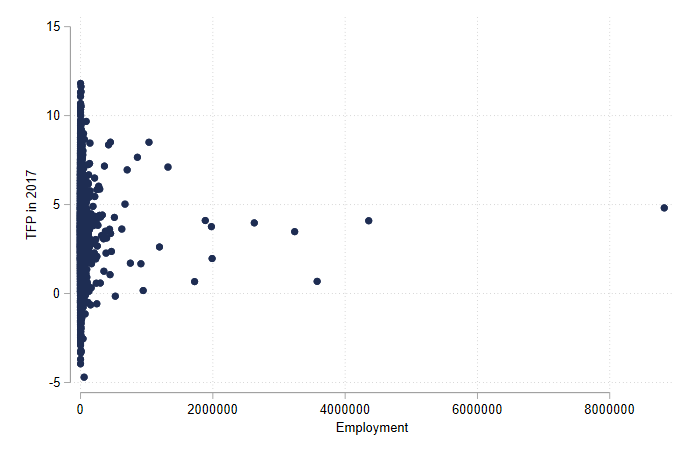
\includegraphics[width=\textwidth]{emp15_outliers}
  	\label{fig:outliers}
\end{figure} 
%---------------------------

To further motivate the use of matching estimators to investigate the effect of FDI on a firm's TFP, the differences in means between the firms that received FDI and the firms that did not are displayed in Table \ref{tab:meandiff1}. The t-tests show significant differences in all observable characteristics, meaning that there is in fact selection into treatment. 

%-------------------------------------TABLE 5
\begin{table}[hbtp!]
	\centering
	\caption{Difference in Pre-Treatment Covariate Means}
	% Balancetable grapvar(FDI2016)

\begin{threeparttable}
\begin{tabular}{lccc}
\\[-1.8ex]\toprule \toprule \\[-1.8ex]
 & (1)  & (2)  & T-test  \\
 & Control  & Treatment  & Difference (1)-(2) \\ \midrule \\[-1.8ex] 
Technology intensity & 2.565 &  1.838 	& 0.728***		\\
				& (0.014) 	& (0.015) 	& 				\\
Access to port 	& 0.273 	& 0.467 	&  -0.194***	\\ 
				& (0.005) 	& (0.007)	& 				\\
Log wages		&  7.529 	& 7.031 	& 0.498*** 		\\ 
				& (0.046)	& (0.057) 	&  				\\
TFP 			& 3.185		& 2.821		& 0.364***		\\ 
				& (0.025) 	& (0.030)  	&				\\
Log employment 	& 3.766 	& 5.405 	& -1.639***		\\
				& (0.037) 	& (0.041)  	&				\\
Log debts 		& 0.511 	& 0.493 	& 0.019***		\\ 
				& (0.004) 	& (0.005)	&			   	\\
Export intensity &  0.131 	&  0.204 	& -0.073*** 	\\ 
				& (0.001) 	& (0.001) 	&				\\
R\&D dummy 		& 0.117 	& 0.128 	& -0.012*		\\ 
				& (0.004) 	& (0.005) 	&  				\\ \\[-1.8ex]
Observations 	& 6863 		& 4460 		&				\\
\bottomrule \bottomrule 
\end{tabular} 

\begin{tablenotes}[flushleft]
\footnotesize
\item \textit{Notes}: Columns (1) and (2) show the pre-treatment covariate means of the control and treatment group respectively. Standard errors are displayed in paratheses. The values displayed for t-tests are the differences in the means across the groups. ***, **, and * indicate significance at the 1, 5, and 10 percent critical level.
\end{tablenotes}

\end{threeparttable}


	\label{tab:meandiff1}
\end{table}
%------------------------------------------


\section{Empirical Specification}

-Overlap?? 

In order to evaluate the causal effect of FDI on Total Factor Productivity (TFP) we estimate our preferred model described in equation (1) using nearest neighbour and nearest neighbour 5 and a caliper of 0.05. Further, we use  inverse probability (IPW) and augmented-inverse probability (AIPW) estimators.
As unlogging employment leaves us better covariate balance we include unlogged employment as a control variable. Further, the inclusion of technology intensity as also exports predict the probability of receiving a treatment too well  [VISUALIZE?]. As propensity score matching requires that all included covariates affect outcome as also treatment variables, we exlude export as latter is likely to solely affect treatment but not our outcome variable. [ADD REFERENCE]. Also, we do not include port due to the same reasoning as before. 

%--------------------------------EQUATION 1
\begin{align*}
TFP  =&  \beta_{0} + \beta_{1} FDI + \beta_{2} X_{i 2015} + \epsilon_{i}   
\end{align*}
where
\begin{itemize}
\item \textit{FDI} is a non-random treatment variable. It takes value 1 in case of treatment, 0 otherwise;
\item  $X_{i 2015}$ describes control variables and consists of following pre-treatment covariates: Ownership, Technology Intensity, Research\&Development, logarithm of Wages, Total Factor Productivity, Employment and Debts
\end{itemize}
%------------------------------------------

The main findings of this paper are displayed in Table \ref{tab:mainresults}. It reports the average treatment effects (ATE) for TFP.  Independent of the estimator, we find highly significant coefficients showing that receiving FDI increases TFP of companies on average. Nonsurprisingly, the reported coefficients differ only slighlty in magnitude. This suggests that our model is not sensitive to different model estimations, which supports our chosen model specification.  Column (1) shows the results of a one-to-one propensity score matching with replacement. Receiving FDI leads for the average company to an increase in TFP of 0.13 standard deviations. Sligthly lower results are obtained from a propensity score matching with five nearest neighbors and a caliper of 0.05 as well as for the invers IPW and AIPW-estimators.
Taking the covariate balances into consideration, we prefer the one-to-one propensity score matching as it gives us bettert covariate balance as compared to the alternative estimators \textit{see Appendix}. Following, we propbe the sensitivity of your findings in  more detail for one-to-one propensity schore matching. 

%-------------------------------------TABLE 6
\subsection{Effect of FDI on TFP}
\begin{table}[h]
 	\centering
   	\caption{ATE of FDI on TFP}
   	\label{tab:mainresults}
\begin{threeparttable}

\begin{tabular}{lcccc} 
	\hline
	\hline
 			& NN1 & NN5\textsuperscript{a} & IPW & AIPW \\
 			& (1) & (2) & (3)  & (4) \\ \hline
 			&  &  &  &    \\
FDI2016 	& 0.130*** & 0.114*** & 0.122***  & 0.122***   \\
 			& (0.015) & (0.011) & (0.007) &   (0.007)  \\
0.FDI2016 	&  &  &  &    \\
P0 Means 	& & & -0.068*** & -0.068***\\
			&  &  & (0.010)  &  (0.010) \\
			&  &  &  &    \\
 Observations & 11,323 & 11,318 & 11,323 & 11,323 \\ 
 	\hline
 	\hline
\end{tabular}

\begin{tablenotes}[flushleft]
      \footnotesize
\item \textit{Note}: Standard errors in parentheses. *** p$<$0.01, ** p$<$0.05, * p$<$0.1.
\item Covariates include, unless otherwise specified: Ownership, Technology Intensity, Research\&Development, logarithm of wages, Total Factor Productivity, Employment and Debts. 
\item All shown coefficients are normalized for better interpretation. 
\item\textsuperscript{a} We use the Propensity Score Matching method with five nearest neihbors and replacement as well as a 0.05 caliper. 
\end{tablenotes}

\end{threeparttable}
\end{table}
%------------------------------------------



\subsection{Robustness of Results}

Table \ref{tab:robust} reports several alternative model specifications that confirm the robustness of our main results. The positive and significant effect of foreign investment on total factor productivity persists. In column (1), we add interaction terms of the dummy variables with the continuous regressors to our set of covariates. The average treatment effect of FDI on productivity slightly increases by 0.027 standard deviations. The covariate balance does not improve with the inclusion of interaction terms, suggesting that interactions do not increase the quality of matching.\footnote{The same holds true when interacting only dummy variables, only continuous variables or all variables.} One possible source of bias are the outliers of employment. While most of the firms' number of employees is concentrated around a mean of 7,111, we are concerned about two observations with extreme values: one firm with over eight million employees, and another one that apparently hired more than 4 million people in 2015.\footnote{Given the limited information our dataset contains, we cannot be sure in which unit employment is measured. We therefore suppose that the common definition of employment being the number of hired employees holds.}  To check whether these outliers influence our main findings, we exclude the two extreme observations. The results reported in column (2) show no significant change in the average treatment effect. %Note% should do F-test for equality of coefficients?%
In our main specification, we have further assumed that a nearby port does not influence total factor productivity. Column (3) confirms that this is indeed the case, as the results do not change with the inclusion of the dummy variable port in our set of covariates. 

%-----------------------TABLE
\begin{table}[h]
  \centering
   \caption{Robustness of Results\textsuperscript{a}}
   \label{tab:robust}
\begin{threeparttable}
 
\begin{tabular}{lcccc} 
	\hline 
	\hline
 		& & & & Effect \\
 		& Including & Excluding & Including & on the\\
 		& Interactions\textsuperscript{b} & Outliers\textsuperscript{c} 
 		& Port\textsuperscript{d} & Treated \\
 		& (1) & (2) & (3) & (4) \\ 
 	\hline
 		&  &  &  &  \\
ATE 	& 0.152*** & 0.127*** & 0.125*** &  \\
 		& (0.016) & (0.015) & (0.019) &  \\
 		&  &  &  &  \\
ATT 	&  &  &  & 0.127*** \\
 		&  &  &  & (0.017) \\
 		&  &  &  &  \\
Observations & 11,323 & 11,321 & 11,323 & 11,323 \\ 
	\hline
	\hline
\end{tabular}

\begin{tablenotes}[flushleft]
     \footnotesize
\item \textit{Note}: Standard errors in parentheses. *** p$<$0.01, ** p$<$0.05, * p$<$0.1.    
     
\item\textsuperscript{a}All specifications use the Propensity Score Matching method with one nearest neighbor and replacement. Covariates include, unless otherwise specified: Ownership, Technology Intensity, Research\&Development, logarithm of Wages, Total Factor Productivity, Employment and Debts. 

\item\textsuperscript{b} Interacting dummy variables (Ownership, Technology Intensity, Research \& Development) with continuous variables (Logarithm of wages, Total Factor Productivity, Employment and Debts).  

\item\textsuperscript{c} Two observations with extreme values of Employment 2015 above four million are excluded.
 
\item\textsuperscript{d} Adding a dummy variable indicating whether a port lies within 500km of the firm to the set of covariates.
\end{tablenotes}

\end{threeparttable}
\end{table}
%--------------------------------------

Finally, column (4) reports the average treatment effect on the treated (ATT) of the nearest neighbor matching with one neighbor and replacement. Because we assume that treatment is not exogenous, we might find stronger effects of treatment on the treated. This would be the case if those firms receiving treatment are also the ones benefiting more from it. However, our estimate in column (4) reports an ATT that is very similar to the average treatment effect for the hypothetical case that all firms have received FDI. This suggests that the propensity score matching performed very well in randomizing treatment and control groups. 

%maybe in conclusion/ limits of paper
One shortcoming of our analysis is the missing capability of explaining the mechanisms behind the observed treatment effects. We do not distinguish between within-firm effects and spillover effects from firms receiving FDI on other firms. Due to the limited information on a firm's sector and location, we are unable to measure spillover effects. That is, the literature on spillover effects typically suggests spillovers within sectors rather than across sectors (SOURCE) and higher spillover effects on nearby firms or firms that are trading factor inputs with foreign-owned companies (SOURCE). 




\section{Analysis by Type}


To further test the robustness of our results  we continue our analysis by looking at potential heterogeneity of the treatment effect across types of FDI. Doing so we can test the possibility that one specific type of Investment drives our previous results. From the data we can distinguish between three different types of FDI: (i) exports-oriented FDI, (ii) technology intensive FDI and (iii) domestic market seeking FDI. Table 5 shows their absolute and relative frequencies. It is possible, that for example only exports-oriented increased factor productivity while the other two types had little or no impact.





To test for this possibility we estimate an augmented IPW model with multi-valued treatment effects. The matching covariates are the same as in the previous model and the regression adjustment specification is the same as that for propensity score estimation. The covariate balance is good, with the highest standardized differences of 5.7\% and a minimum variance ratio of 0.55 for employment (though all other variance ratios are close to 1).

Second, we estimate an IPW model to check if it yields similar estimates without regression adjustment. The covariate balance in this model is practially the same. Finally, we estimate a set of AIPW models where we restrict the sample to one type of treatment each. This allows for the IIA assumption to be relaxed which is required for the Mulitnomial Logit model. The first logit model has a maximum standardized difference of 12\% for employment and and a maximum variance ratio of 1.36 for the same variable. The second model fares better in terms of standardized differences but has has a variance ratio of 1.88 for employment. The third model has great balance in all variables. The overlap assumption is satisfied for all treatment levels as can be seen in graph \ref{fig:psbytype}. 


In Table \ref{tab:bytype} the results from the typewise analysis are shown. In the AIPW Multinomial specification the differences in ATE between different types of FDI are below half a percent of a standard deviation. This suggests, that all types of FDI increase factor productivtiy by essentially the same margin. The estimated effect size is close to the one estimated for FDI in tabl 2. In the IPW specification the differences are a bit larger but no bigger than 4.5\% of a standard deviation. The seperate logit models also yield essentially the same effect sizes as the multinomial specification. We thus conclude that all types of FDI increase productivity by 

The Inverse Probability Weighting Model gives us somewhat bigger differences in effect sizes between the types. The difference between the bigger effect of Exports oriented FDI and the smaller effect of Technology intensive FDI amounts to 4\% of a standard deviation. Including interaction terms between continuous and categorical regressors 

With the AIPW being a doubly robust estimators and rather small differences in the IPW estimator we take these results to suggest that all types of FDI have similar positive impacts on factor productivity. 

%-----------------------------TABLE
\begin{table}[htbp]
	\centering
	\caption{ATE by Type of FDI}
	\label{tab:bytype}
\begin{threeparttable}

\begin{tabular}{lccccc} 
		\hline
		\hline
 	& (1) & (2) & (3) & (4) & (5) \\
	& AIPW & IPW  & AIPW  & AIPW & AIPW \\ 
	& Mlogit & Mlogit &Logit &Logit &Logit\\
		\hline
 			&  &  &  &  &   \\
Exports-oriented FDI 	& 0.144*** &   0.157*** & 0.140*** &  &  \\
 						& (0.006) &   (0.032) & (0.007) &  &\\
Technology intensive FDI & 0.139***   & 0.112*** &  & 0.139*** &   \\
 						 & (0.005)  & (0.018) &  &  (0.005)&  \\
Domestic market seeking FDI & 0.143*** &   0.134*** &  &  &0.143*** \\
 							& (0.004)   & (0.011) &  &  & (0.004)  \\
PO Means 		&   -0.057*** &   -0.068*** &-0.012  &-0.025**  & -0.017    \\
 				&   (0.009) &   (0.010) &  (0.011)&(0.011)  & (0.011) \\
Observations 	& 11,323  & 11,323 &  7,803  & 8,418 & 8,828  \\ 
		\hline
		\hline
\end{tabular}

\begin{tablenotes}[flushleft]
	\footnotesize
\item \textit{Note}: Robust standard errors in parentheses. *** p$<$0.01, ** p$<$0.05, * p$<$0.1.
\end{tablenotes}

\end{threeparttable}
\end{table}
%------------------------------------------------

To account for the possibility that the choice of the FDI type does not satisfy the IIA assumption we further estimate separate logit models for the two estimator types. The results, reported in table 7, are very similar to those obtained from a multinomial specification, suggesting that the IIA assumption holds.  

%-------------------FIGURE 
\begin{figure}[h]\centering
\caption{Propensity Score by Treatment Level}
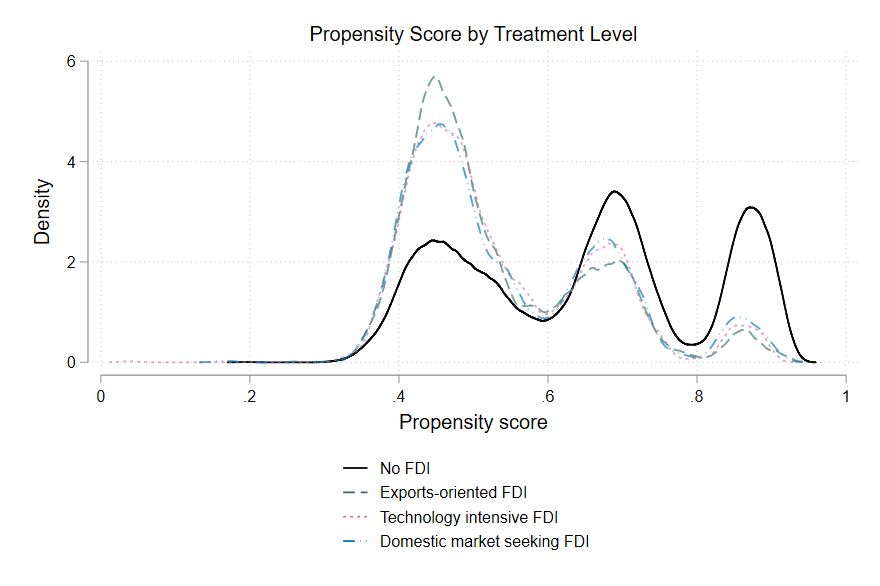
\includegraphics[height=11cm]{mlog_overl_ppb.png}\\[0.5cm] 
\label{fig:psbytype}
\end{figure}
%------------------------


\section{Discussion/Conclusion}
For citation: \\
you have to add your reference firstly in bibCG. After having done so you can always include the reference in the actual file as follows: \\
 \citet{biddle1990sleep}\\
\citep[p.~35]{CaliendoHujerThomsen2008}	 \\


Thoughts on what we could write for discussion/limits of our study: 
\begin{enumerate}
\item Do not know much about the context of the treatment (so cannot really rule out anticipation-effects?)
\item Would have been interesting to extend the study to several years after the treatment. Do effects persist? Do they vanish? 
\item Might depend on firm size (see Aitken \& Harrison 1999 $\rightarrow$ will include citation): find positive within-plant effects and spillover effects on TFP for small firms only (less than 50 employees)
\item Do not measure spillovers on plants that have not received FDI
\item Do not have sector-specific data $\rightarrow$ TECH variable has only 4 categories; e.g. in order to measure spillover effects from other firms in sector this would be necessary (i.e. if a foreign firm is more innovative)
\end{enumerate}


\newpage

%-------------------------------------------------------------
% References
%-------------------------------------------------------------
\addcontentsline{toc}{section}{References}	%Adds references to table of contents
\bibliography{bibCG} 
\newpage


%-------------------------------------------------------------
% Appendix
%-------------------------------------------------------------

\section*{Appendix}
\pagenumbering{roman}
\sectionnumbering{Roman}
\setcounter{page}{3} %May have to adjust this if we leave out list of tables or add something else

\end{document}